\begin{titlepage}

  
  %%Logo
  \DeclareNewLayer[
  align=tl,
  hoffset=0cm,
  voffset=0cm,
  width=4cm,
  height=2.2cm,
  background,
  contents={
\includegraphics[width=\layerwidth]{~/.emacs.d/templates/image/dg_d.png}}
  ]{logo}

  %% Footer
  \DeclareNewLayer[
  align=tl,
  hoffset=0cm,
  voffset=27cm,
  width=21cm,
  height=2.2cm,
  background,
  contents={
\includegraphics[width=\layerwidth]{~/.emacs.d/templates/image/dg_footer.png}}
  ]{footer}

  %% Adressfeld
  \DeclareNewLayer[
  align=tl,
  hoffset=4cm,
  voffset=25.5cm,
  width=5cm,
  height=3\baselineskip,
  contents={
	\footnotesize{
      \begin{flushleft}
        \textbf{duagon AG} \newline
        Riedstrasse 12     \newline
        8953 Dietikon
      \end{flushleft}}
  }
  ]{addressfield}

  %% www
  \DeclareNewLayer[
  align=tl,
  hoffset=4cm,
  voffset=27.4cm,
  width=5cm,
  height=1\baselineskip,
  contents={
	\begin{flushleft}
      \footnotesize www.duagon.com
      \end{flushleft}
  }
  ]{www}

%% Docoration Image
  \DeclareNewLayer[
  align=tl,
  hoffset=6cm,
  voffset=15cm,
  width=12cm,
  height=12cm,
  background,
  contents={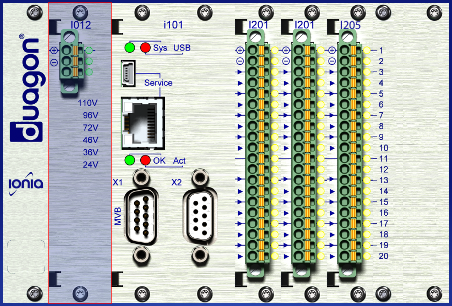
\includegraphics[width=\layerwidth]{~/.emacs.d/templates/image/dg_deco.png}}
  ]{deco}
  
  \vspace*{-1cm}
  \Huge{
      \begin{center}
        \textsf{\textcolor{DG_YELLOW} {Title and Some More Words does it make line brake?}}
      \end{center}}

  \vspace*{0.5cm}
  \huge{
      \begin{flushleft}
        \textrm{Technical Note}
      \end{flushleft}}

 \vspace*{1cm}
  \large{
      \begin{flushleft}
        \textrm{Some short description of the paper}
      \end{flushleft}}
  
  \DeclareNewPageStyleByLayers{titlestyle}{logo,deco,footer,addressfield,www}
  \thispagestyle{titlestyle} %% Logo in header
\end{titlepage}
